% Dokument-Typ festlegen
\documentclass[titlepage,abstracton,headsepline, footsepline, a4paper,BCOR=8.25mm, DIV=15]{scrartcl}

% Unterst�tzung f�r Deutsch einbinden
%\usepackage[ngerman]{babel}

% Pakete f�r die Darstellung und Eingabem�glichkeit von Umlauten
%\usepackage[T1]{fontenc}
%\usepackage[ansinew]{inputenc}

% Farben nutzen
\usepackage{xcolor}
\definecolor{darkgreen}{rgb}{0,130,0}

%\usepackage[bookmarks=true,pdfborder={0 0 0}]{hyperref}

 \usepackage{listings}
  \usepackage{courier}
 \lstset{
		 commentstyle=\tiny\ttfamily\color{black},
         basicstyle=\tiny\ttfamily, % Standardschrift
         %commentstyle=\fontsize{12}{14.4}\selectfont,
         %basicstyle=\ttfamily\fontsize{10}{12}\selectfont
         %numbers=left,               % Ort der Zeilennummern
         %numberstyle=\tiny,          % Stil der Zeilennummern
         %stepnumber=2,              % Abstand zwischen den Zeilennummern
         numbersep=3pt,              % Abstand der Nummern zum Text
         tabsize=2,                  % Groesse von Tabs
         extendedchars=true,         %
         breaklines=true,            % Zeilen werden Umgebrochen
         keywordstyle=\bfseries\ttfamily\color{orange},
         stringstyle=\color{darkgreen}\ttfamily,
         emph={rmc, gps_buffer_rmc},
         emphstyle=\color{blue}\texttt,
         %keywordstyle=\color{red}\textbf,
    	%	frame=b,         
         %keywordstyle=[1]\textbf,    % Stil der Keywords
         %keywordstyle=[2]\textbf,    %
         %keywordstyle=[3]\textbf,    %
         %keywordstyle=[4]\textbf,   %\sqrt{\sqrt{}} %
         %stringstyle=\color{white}\ttfamily, % Farbe der String
         showspaces=false,           % Leerzeichen anzeigen ?
         showtabs=false,             % Tabs anzeigen ?
         xleftmargin=17pt,
         framexleftmargin=17pt,
         framexrightmargin=5pt,
         framexbottommargin=4pt,
         %backgroundcolor=\color{lightgray},
         showstringspaces=false      % Leerzeichen in Strings anzeigen ?        
 }
 \lstloadlanguages{% Check Dokumentation for further languages ...
         %[Visual]Basic
         %Pascal
         C
         %C++
         %XML
         %HTML
         %Java
 }
%\DeclareCaptionFont{blue}{\color{blue}} 

%\captionsetup[lstlisting]{singlelinecheck=false, labelfont={blue}, textfont={blue}}
\usepackage{caption}
\DeclareCaptionFont{white}{\color{white}}
\DeclareCaptionFormat{listing}{\colorbox[cmyk]{0.43, 0.35, 0.35,0.01}{\parbox{\textwidth}{\hspace{15pt}#1#2#3}}}
\captionsetup[lstlisting]{format=listing,labelfont=white,textfont=white, singlelinecheck=false, margin=0pt, font={bf,footnotesize}}

\usepackage{listings} 
\lstset{numbers=left, numberstyle=\tiny, numbersep=5pt} 
\lstset{language=Matlab}
\lstset{basicstyle={\ttfamily\small}}
\lstset{keywordstyle={\color{blue}}, backgroundcolor={\color{white}}, frame={shadowbox}, commentstyle={\color{darkgreen}}}

% Autoren und Titel definieren
\author{Armin Schlegel,\\Christian Eismann}
\title{GPS Bycicle Computer} 

\usepackage{graphicx}
\pagestyle{headings} 
% \fontfamily{phv}

\usepackage{longtable}
\usepackage{caption}
\setcounter{secnumdepth}{3}

\begin{document}
\maketitle
\tableofcontents
\newpage
\listoffigures
\newpage
\begin{abstract}
This document contains the description and API specification of the project \textit{GPS Bicycle computer}. The target of this project
was to create an electronic mobile device that provides several informations on an graphic display. The actual information is determined
by analyzing different data sets provided by a GPS receiver. Further more an SD card controller enables data recording on a SD card. An
overview of the general functionality is shown in figure \ref{general_info}. 

\begin{minipage}[t]{\textwidth}
\centering
\includegraphics[width=\textwidth]{general_functionality.pdf}
\captionof{figure}[General functionality]{General functionality}
\label{general_info}
\end{minipage}\\
\end{abstract}

\section{Introduction}
In this chapter the basic features (must-have features) are introduced.

\subsection{The main features}
\begin{itemize}
\item{\textbf{Receiving and processing of GPS data}\\
The information that is provided to the user is determined by analyzing received GPS data sets. Information about latitude/longitude, data
time and several more can be provided.}
\item{\textbf{Visualization of GPS data on a graphic display}\\
The already mentioned data is then presented on a graphic display to the actual user.}
\item{\textbf{Storing of received data}\\
The data provided by the GPS receiver can be recorded to a SD card. In further processing this can be used, for example, to analyze a road trip
with Google Earth.}
\item{\textbf{Charging electronics}\\
The charging electronics is required for recharging used batteries.}
\end{itemize}
\section{The toolchain}
In this chapter all tools that have been used during this project are described. Furthermore tools that could have been used alternatively are
also noted.
\subsection{Hardware development tools}
For the hardware development, that means circuit board design and layout, only EAGLE from Cadsoft has been used.\\

\subsection{Software development tools}
The main target was to assemble a toolchain containing open-source tools only. Especially for the AVR ATmega series a lot of open source alternatives
to the AVR Studio IDE exists. By using these tools a mostly automatic toolchain can be assembled. Another possibility would be using eclipse
with a special AVR plugin (\texttt{The AVR Eclipse Plugin}).

\subsubsection{Oracle Virtualbox}
The base for the toolchain used within this project is Linux. However, doing software development on a Linux distribution involves several
complications in most cases. An appropriate alternative would be CygWin, an open source terminal for Windows that emulates the Linux API. Nearly
all Linux standard tools are supported by CygWin, such as grep, find, gcc, gdb, ... . But obviously it is dependent on the Windows version in which it is installed on.
For example Windows 7 is not fully supported yet. So for implementing a Linux based toolchain a virtual machine is used, that can be simply copied 
to any PC for further developing. Virtualbox from Oracle is the best choice in this context, because it is freeware and, in opposite to the VM 
Player from VMware, virtual machine images can be created. Furthermore it supports access to the file system of the parent OS (e.g. Windows). So 
it is very easy to share data between both operating systems. The Linux distribution running
on the machine is a Debian image (pretty small, but contains all necessary tools). By using the apt-get shell functionality further tool 
installing is very comfortable. (e.g. for installing grep, simply type: apt-get install grep).

\subsubsection{The GNU Compiler Collection (AVR-GCC)}
The main component of this toolchain is the AVR-GCC, containing compiler, linker, debugger and so on. The AVR-GCC is a port of the original GNU 
GCC, so there is a well reviewed documentation available for all tools. Even a ported version of the LIBC is available for AVR microcontroller 
development. The free compiler suit is one of the biggest advantages of AVR microcontrollers for projects like the GPS bycicle computer. Actually 
compilers for microcontrollers from other vendors are mostly very expensive (e.g. CodeWarrior from Freescale).

\subsubsection{The Programmer: avrdude}
To actually program the target avrdude is used. This tool is also open source and freeware. Furthermore, like all other previous mentioned Linux tools, it can be called
via Makefiles. Avrdude supports various hardware programmers.

\subsubsection{Make}
Make is \textbf{the} standard tool for managing and building binaries and libraries from source code.

\subsubsection{(Sp)lint}
Splint is a static code analysis tool for the C Programming Language. In this project it has been used for advanced failure tracking. But obviously this tool reports
too many positive faults for continuous usage within a project. Furthermore the tool actually explain the user how to disable certain warnings. Therefore it is even in
a professional project not recommendable.\\
Instead of using splint any further we decided to extend the warning options of the AVR-GCC compiler.\\
\begin{minipage}[t]{\textwidth}
\centering
\lstinputlisting[language=make,label=gcc_compiler_warnings,caption=GCC compiler warnings]{Makefile_warnings.mak}
\label{gcc_warnings}
\end{minipage}\\


\section{Hardware development}
Before we began with the hardware design it became necessary to analyse the components we needed. 
\subsection{Requirement analysis and pre-selection of hardware components}

\begin{longtable}{|p{3.2cm}|p{3.4cm}|p{3cm}|p{3cm}|}
\hline
\textbf{Component} &
\textbf{Details} &
\textbf{Why this component?} &
\textbf{Comment}\\
\hline
ATMega32-L &
8-Bit, \textbf{3.3V}, 32kB Flash, 2kB SRAM, 4kB EEPROM &
Runs on 3.3V,easy to program via GNU GCC and other GNU Tools &
Became obsolete due a lack of RAM\\
\hline
ATMega664-L &
Pin compatible to the ATMega32-L, 64kB Flash, \textbf{4kB SRAM} &
Has 2kB more RAM than the old CPU needed by the application &
Used as CPU after lack of RAM\\
\hline
NL-552ETTL &
GPS-Receiver, 5V supply, \textbf{RS232} communication with \textbf{3.3V TTL} &
Supports NMEA, supports european GALLILEO sattelites, 3.3V levels makes level shifting unnecessary &
 \\
\hline
MAX3221 &
\textbf{3.3V}, RS232 driver &
e.g. for debugging on a PC &
Never used\\
\hline
LM 2940 &
5V Low Dropout Regulator &
Can use min. 5.5V to generate 5.0V &
Discharges the batteries to 5.5V\\
\hline
LT1117-3.3 &
\textbf{3.3V} Drouput Regulator &
3.3V needed for CPU, SD-Card, Display, RS232 Driver &
 \\
\hline
EA-DOGL128W, EA-LED68x51-W, EA-TOUCH128-2 &
\textbf{3.3V}, \textbf{SPI}, 128x64 b/w, white backgroundlight, touch &
Cheap, easy to use via SPI, backlight and touchscreen available &
Consumes approx. 80mA\\
\hline
Yamaichi FPS009-2305 &
Slot for SD-Cards, can be read out if card is present and writeable or locked &
It was the cheapest &
 \\
\hline
LEDs &
 &
Some user LEDs &
 \\
\hline
JTAG &
 &
programming and debugging &
 \\
\hline
ISP &
 &
programming &
 \\
\hline
\end{longtable}

\subsection{Layout and design}
Because of the lack of time we jumped over a first prototype board and went directly to the attempt to create the final prototype hardware. We 
wanted the project to be compact and portable so the first thought was to bring the complete hardware design down to SMD components. In second 
thoughts to make the device tiny and portable, a compact design is needed. So we decided to put one circuit board on top of another connected via 
plug connectors.

As the project contains a graphical display its obvious that it has to be placed on top. Because the display and 
the SD-card communicates with the processor via SPI it is convenient to combine both on one circuit board. It is useful to place the user LEDs on 
the top too. This board is called the ``displayboard" and is connected on top of the ``mainboard".

The ``mainboard" contains the rest of the components like CPU, JTAG and ISP connectors, voltage regulators, etc.
In order to get the device mobile there are some batteries needed. We chose five AAA 1.2V rechargeable batteries because they are easy to 
recharge. If all batteries are completely charged (at 1.4V each) the resulting voltage is 7.0V. This is the maximum Voltage the batteries can 
deliver. At the minimum of 5.5V (1.1V each battery) the 5V Regulator quits and the batteries won't discharge further. This will prevent the 
batteries from total discharge that would cause severe damage to the batteries.

To get the device stay longer alive we thought about a opportunity to charge the batteries while driving. For example this could be done hub 
generator.
In order to charge the batteries to the maximum of 7V a regulator is needed that generates 7V out of the hub generator voltage. Therefore a 
``supplyboard" was built.

The ``supplyboard" contains a combined step-up and step-down regulator (SEPIC) in order to generate the needed 7 V out of the voltage coming from the hub dynamo with the range of 4 to 40 Volt AC.

\begin{minipage}[t]{\textwidth}
\centering
\includegraphics[width=\textwidth]{blockschaltbild.pdf}
\captionof{figure}[Hardware Block Diagram]{Hardware Block Diagram}
\label{block_diagram}
\end{minipage}\\

Within figure \ref{block_diagram} the hardware components of the entire product and the relations between them is shown.

\begin{minipage}[t]{\textwidth}
\centering
\includegraphics[width=\textwidth]{mainboard_schaltplan.pdf}
\captionof{figure}[Mainboard schematics]{Mainboard schematics}
\label{mainboard_schematics}
\end{minipage}\\

\begin{minipage}[t]{\textwidth}
\centering
\includegraphics[width=\textwidth]{mainboard_layout.pdf}
\captionof{figure}[General functionality]{General functionality}
\label{mainboard_layout}
\end{minipage}\\

\begin{minipage}[t]{\textwidth}
\centering
\includegraphics[width=\textwidth]{displayboard_schaltplan.pdf}
\captionof{figure}[Displayboard schematics]{Displayboard schematics}
\label{displayboard_schematics}
\end{minipage}\\

\begin{minipage}[t]{\textwidth}
\centering
\includegraphics[width=\textwidth]{displayboard_layout.pdf}
\captionof{figure}[Displayboard layout]{Displayboard layout}
\label{displayboard_layout}
\end{minipage}\\

\begin{minipage}[t]{\textwidth}
\centering
\includegraphics[width=\textwidth]{supplyboard_schaltplan.pdf}
\captionof{figure}[Supplyboard schematics]{Supplyboard schematics}
\label{supplyboard_schematics}
\end{minipage}\\

\begin{minipage}[t]{\textwidth}
\centering
\includegraphics[width=\textwidth]{supplyboard_layout.pdf}
\captionof{figure}[Supplyboard layout]{Supplyboard layout}
\label{supplyboard_layout}
\end{minipage}\\

\section{Software development}
In this chapter the software development which was done during this project is described. In addition to that all API functions are mentioned in the following sections.

\subsection{Software Pre-Analysis}
For transmitting GPS data from the receiver to any microcontroller (or any other processing unit) the \texttt{``National Marine Electronics 
Association"} (NMEA) protocol is used. NMEA is an ASCII based protocol, used for transmitting \texttt{character frames} from one participant
to another. The general structure of a NMEA frame is shown in figure \ref{NMEA_protocol}.

\begin{minipage}[t]{\textwidth}
\centering
\includegraphics[width=0.5\textwidth]{NMEA_protocol.pdf}
\captionof{figure}[NMEA protocol structure]{NMEA protocol structure}
\label{NMEA_protocol}
\end{minipage}\\

For the configuration of the GPS receiver UBX (acronym for \texttt{U-Blox}) protocol messages are used. The proprietary UBX format is shown
in figure \ref{ubx_protocol}.

\begin{minipage}[t]{\textwidth}
\centering
\includegraphics[width=0.5\textwidth]{ubx_protocol.pdf}
\captionof{figure}[UBX protocol structure]{UBX protocol structure}
\label{ubx_protocol}
\end{minipage}\\

For further detailed information about these protocols please refer to the according data sheet of the U-Blox 5.

\subsection{General design}
General spoken a project providing a more or less complex user interaction via a graphical touch display usually requires the implementation of 
an Operating System. But obviously this work would be too time consuming for such a small project like this. So we decided to abandon on extended 
touch screen functionality in a first step. As consequence the general workflow is kept as simple as possible.

\subsection{Program workflow}
After initializing every component like spi, display driver, uart and others the central part of the program control is an infnite while loop within the main routine. 
The actual application is triggered on every \texttt{SIG\_USART\_RECV} interrupt request. 
This IRQ indicates that the GPS receiver has sent new data to the microcontroller via UART. 
Figure 8 visualizes the basic functionality: most of the runtime the microcontroller is waiting for incoming data (\texttt{SIG\_USART\_RECV}). 
Every time the interrupt is thrown one byte has been read from the UART interface as long as all needed GPS blocks are completely received.
This is monitored with the aid of the identifier tags of the NMEA tags like \texttt{\$GPRMC} or \texttt{\$GMVTG}.
The received data is stored within a separate buffer (\texttt{char uart\_str[]}) and then split up to its separate components (\texttt{RMC, VTG and GGA}
data sets). 
If all conditions for recording are met (at least 3 sattelites, SD card present and writeable) the user can start a record via the touchscreen.
If the user set the device to record the whole \texttt{uart\_str[]} buffer is stored on a SD Card.
In order to display the correct data, some calculations are done. Those calculations where for example to convert the \texttt{NMEA} format of longitude and latitude in a human readable format 
or correct the view of the time. 
After all the wanted information is being displayed.

\begin{minipage}[t]{\textwidth}
\centering
\includegraphics[width=\textwidth]{interrupt_function.pdf}
\captionof{figure}[General workflow overview]{General workflow overview}
\label{interrupt_function}
\end{minipage}\\

\subsection{Modules}
This section provides an overview about the functionality within the separate software modules. The API function documentation can be found in the
delivered tar-ball (generated by using doxygen).

\subsubsection{Display}
As described in the data sheet of the graphic display, the data transmission between the display and the CPU is unidirectional. In consequence
to this, the current set pixels have to be stored in CPUs SRAM to avoid loosing the actual frame information.

The \textit{Display} module provides the following features:
\begin{itemize}
\item \textbf{\underline{Sending data to the display}}\\
This functionality is mandatory for the general handling of the graphic display. The implemented methods provides an interface for sending 
commands (e.g. turn display on) and data (e.g. an entire frame) via \texttt{SPI}. 
\item \textbf{\underline{Initialization of the graphic display}}\\
The actual hardware initialization. As described in the data sheet of the EA DOGL 128L (\cite{EADOGL}) different preferences have to be configured
before using the display, such as display contrast, starting line, etc.
\item \textbf{\underline{Writing text}}\\
The byte representation of every single character is stored within the \texttt{Font5x7[]} array (in EEPROM). To write text to the display the index
of the required character is determined. Taken the data from that array and sending it to the display by using the \texttt{display\_putpixel()}
function results in a printed character on the graphical display.
\item \textbf{\underline{Painting pictures}}\\
For painting a picture e.g. a bitmap file has to be converted to a representing byte array. The provided tool ``GrafikKonverterV1\_1" provides 
this functionality.
\end{itemize}

As an example for the internal pixel representation the following listing shows the sending of an entire frame to the display controller.\\
\begin{minipage}[t]{\textwidth}
\centering
\lstinputlisting[language=c,label=sending_frame,caption=Sending a frame to the display controller]{SendFrame.c}
\label{sending_frame}
\end{minipage}\\

\subsubsection{GPS}
Within this module the actual resolving of GPS data sets is realized. Furthermore the storage of GPS data to the SD card is implemented.
The central functionality of the GPS module is the actual splitting of GPS data sets into separate tokens. This is done in function
\texttt{gps\_split\_data()}. First the type of the current received data set is determined. For each different type a separate splitting
function is implemented (\texttt{gps\_split\_gga(), gps\_split\_rmc(), gps\_split\_vtg()}. Within these functions a data set is split into its
tokens, separated by ``," or ``*". In a next step these tokens are stored in the according data buffer (\texttt{rmc[], gga[] or vtg[]}).

As shown in listing 2 every single data component of a RMC, GGA or VTG data set is separated by a single comma. Only
the checksum at the end of the NMEA frame is separated by a ``*".

\begin{minipage}[t]{\textwidth}
\centering
\lstinputlisting[label=nmea_data_sets_example,caption=Example of NMEA data sets]{NMEAexample.txt}
\label{nmea_data_sets_example}
\end{minipage}\\

The static PUBX messages used for initializing the GPS receiver are stored within EEPROM to avoid a waste of RAM memory.

\begin{minipage}[t]{\textwidth}
\centering
\lstinputlisting[language=c,label=static_gps_init,caption=Static GPS initialization PUBX commands]{StaticGPSInit.c}
\label{static_gps_init}
\end{minipage}\\

\subsubsection{Interrupt}
In this module the main interrupt routine is implemented, that is triggered as soon as a new byte has been received via UART from the GPS 
receiver. A detailed visualization of this functionality is shown in figure \ref{interrupt_function}.

\subsubsection{SPI}
In this module the SPI driver is implemented. This includes the initialization (\texttt{spi\_init()}), the sending of single bytes
(\texttt{spi\_send()}) and the reading of single bytes from the SPI (\texttt{spi\_read()}).
\subsubsection{UART}
This module realizes the serial data communication between the GPS receiver unit and the microcontroller. This includes initialization of UART 
and receiving/sending of single bytes. One part of the initialization is the setting of the baudrate to 38400 (\texttt{uart\_init\_high()}). 
If the GPS receiver has still its default settings the communication between the microcontroller and the GPS receiver is only possible with a baudrate of 38400.
After initializing the GPS receiver and setting its baudrate to 9600, the baudrate of the UART has to be set to 9600 too in order to keep up the communication.
(\texttt{uart\_init\_low()}). 

The high baudrate of 38400 is actually not necessary for the general communication between GPS receiver and microcontroller, because the 
processing time (data processing, display output, SD output) is so short, that in this case a lower baudrate is preferred. 
Another reason to have a low baudrate is that it's also applicable for communication between microcontroller and a PC (high baudrate causes short transmission range).

\subsection{SDC/Fat16}
The SDC/Fat16 modules are external libraries. Only in SDC some IO functionality has been adapted.

\subsection{The application}
The actual application is placed within the s.c. "Windows" module. Here the already prepared GPS data is converted into the different
standardized representations. In function \texttt{window1()} the actual display output is controlled. Several helper functions provides easy
access to the corresponding representations of the GPS data. The \texttt{window1()} function is triggered by every incoming \texttt{SIG\_USART\_RECV} (see also \texttt{interrupt.c}) interrupt, as soon as a data block has been completly processed.

\section{User Guide}
\subsection{Turn on power supply.}
The ``Power ON/OFF" switch can be found on the right side of the product. Figure \ref{PIC_power_on} shows that switch and the SD card slot.\\\\
\begin{minipage}[t]{0.7\textwidth}
\centering
\includegraphics[width=\textwidth]{PIC_power_on.pdf}
\captionof{figure}[Power ON/OFF Switch]{Power ON/OFF Switch}
\label{PIC_power_on}
\end{minipage}\\

\subsection{Display layout}
The general layout of the display is shown in figure \ref{PIC_layout}.\\
\begin{minipage}[t]{\textwidth}
\centering
\includegraphics[width=\textwidth]{PIC_layout.pdf}
\captionof{figure}[General display layout]{General display layout}
\label{PIC_layout}
\end{minipage}\\

\subsection{Recording data to SD card}
\textbf{Precondition:} A SD card has to be provided to the SD card slot.\\
For recording NMEA data to a SD card, simply push on the graphical display for at least three seconds. As soon as recording starts a status picture
will inform you about the beginning of data recording as shown in figure \ref{PIC_record_init}. Figure \ref{PIC_record} shows the display during a record. The recording is signalized by the small circle that is alternating filled and unfilled. To stop recording, simply touch on the display 
for three seconds again.\\\\
\textbf{Note:} Before recording the SD card has to be formatted to the \texttt{FAT16} format. For doing this with a Linux distribution use the command ``\texttt{mkfs.vfat -F 16 -S512 /dev/sdXY}" (\texttt{sdXY} is the identifier for your SD card) on a terminal. On a PC running Windows simply format the SD card with FAT16 format and a block size of 512Byte (Note: this has not been tested). \textbf{The formating is mandatory for recording data.}\\\\
\begin{minipage}[t]{0.5\textwidth}
\centering
\includegraphics[width=\textwidth]{PIC_record_init.pdf}
\captionof{figure}[Record Initialization status message]{Record Initialization status message}
\label{PIC_record_init}
\end{minipage}
\begin{minipage}[t]{0.5\textwidth}
\centering
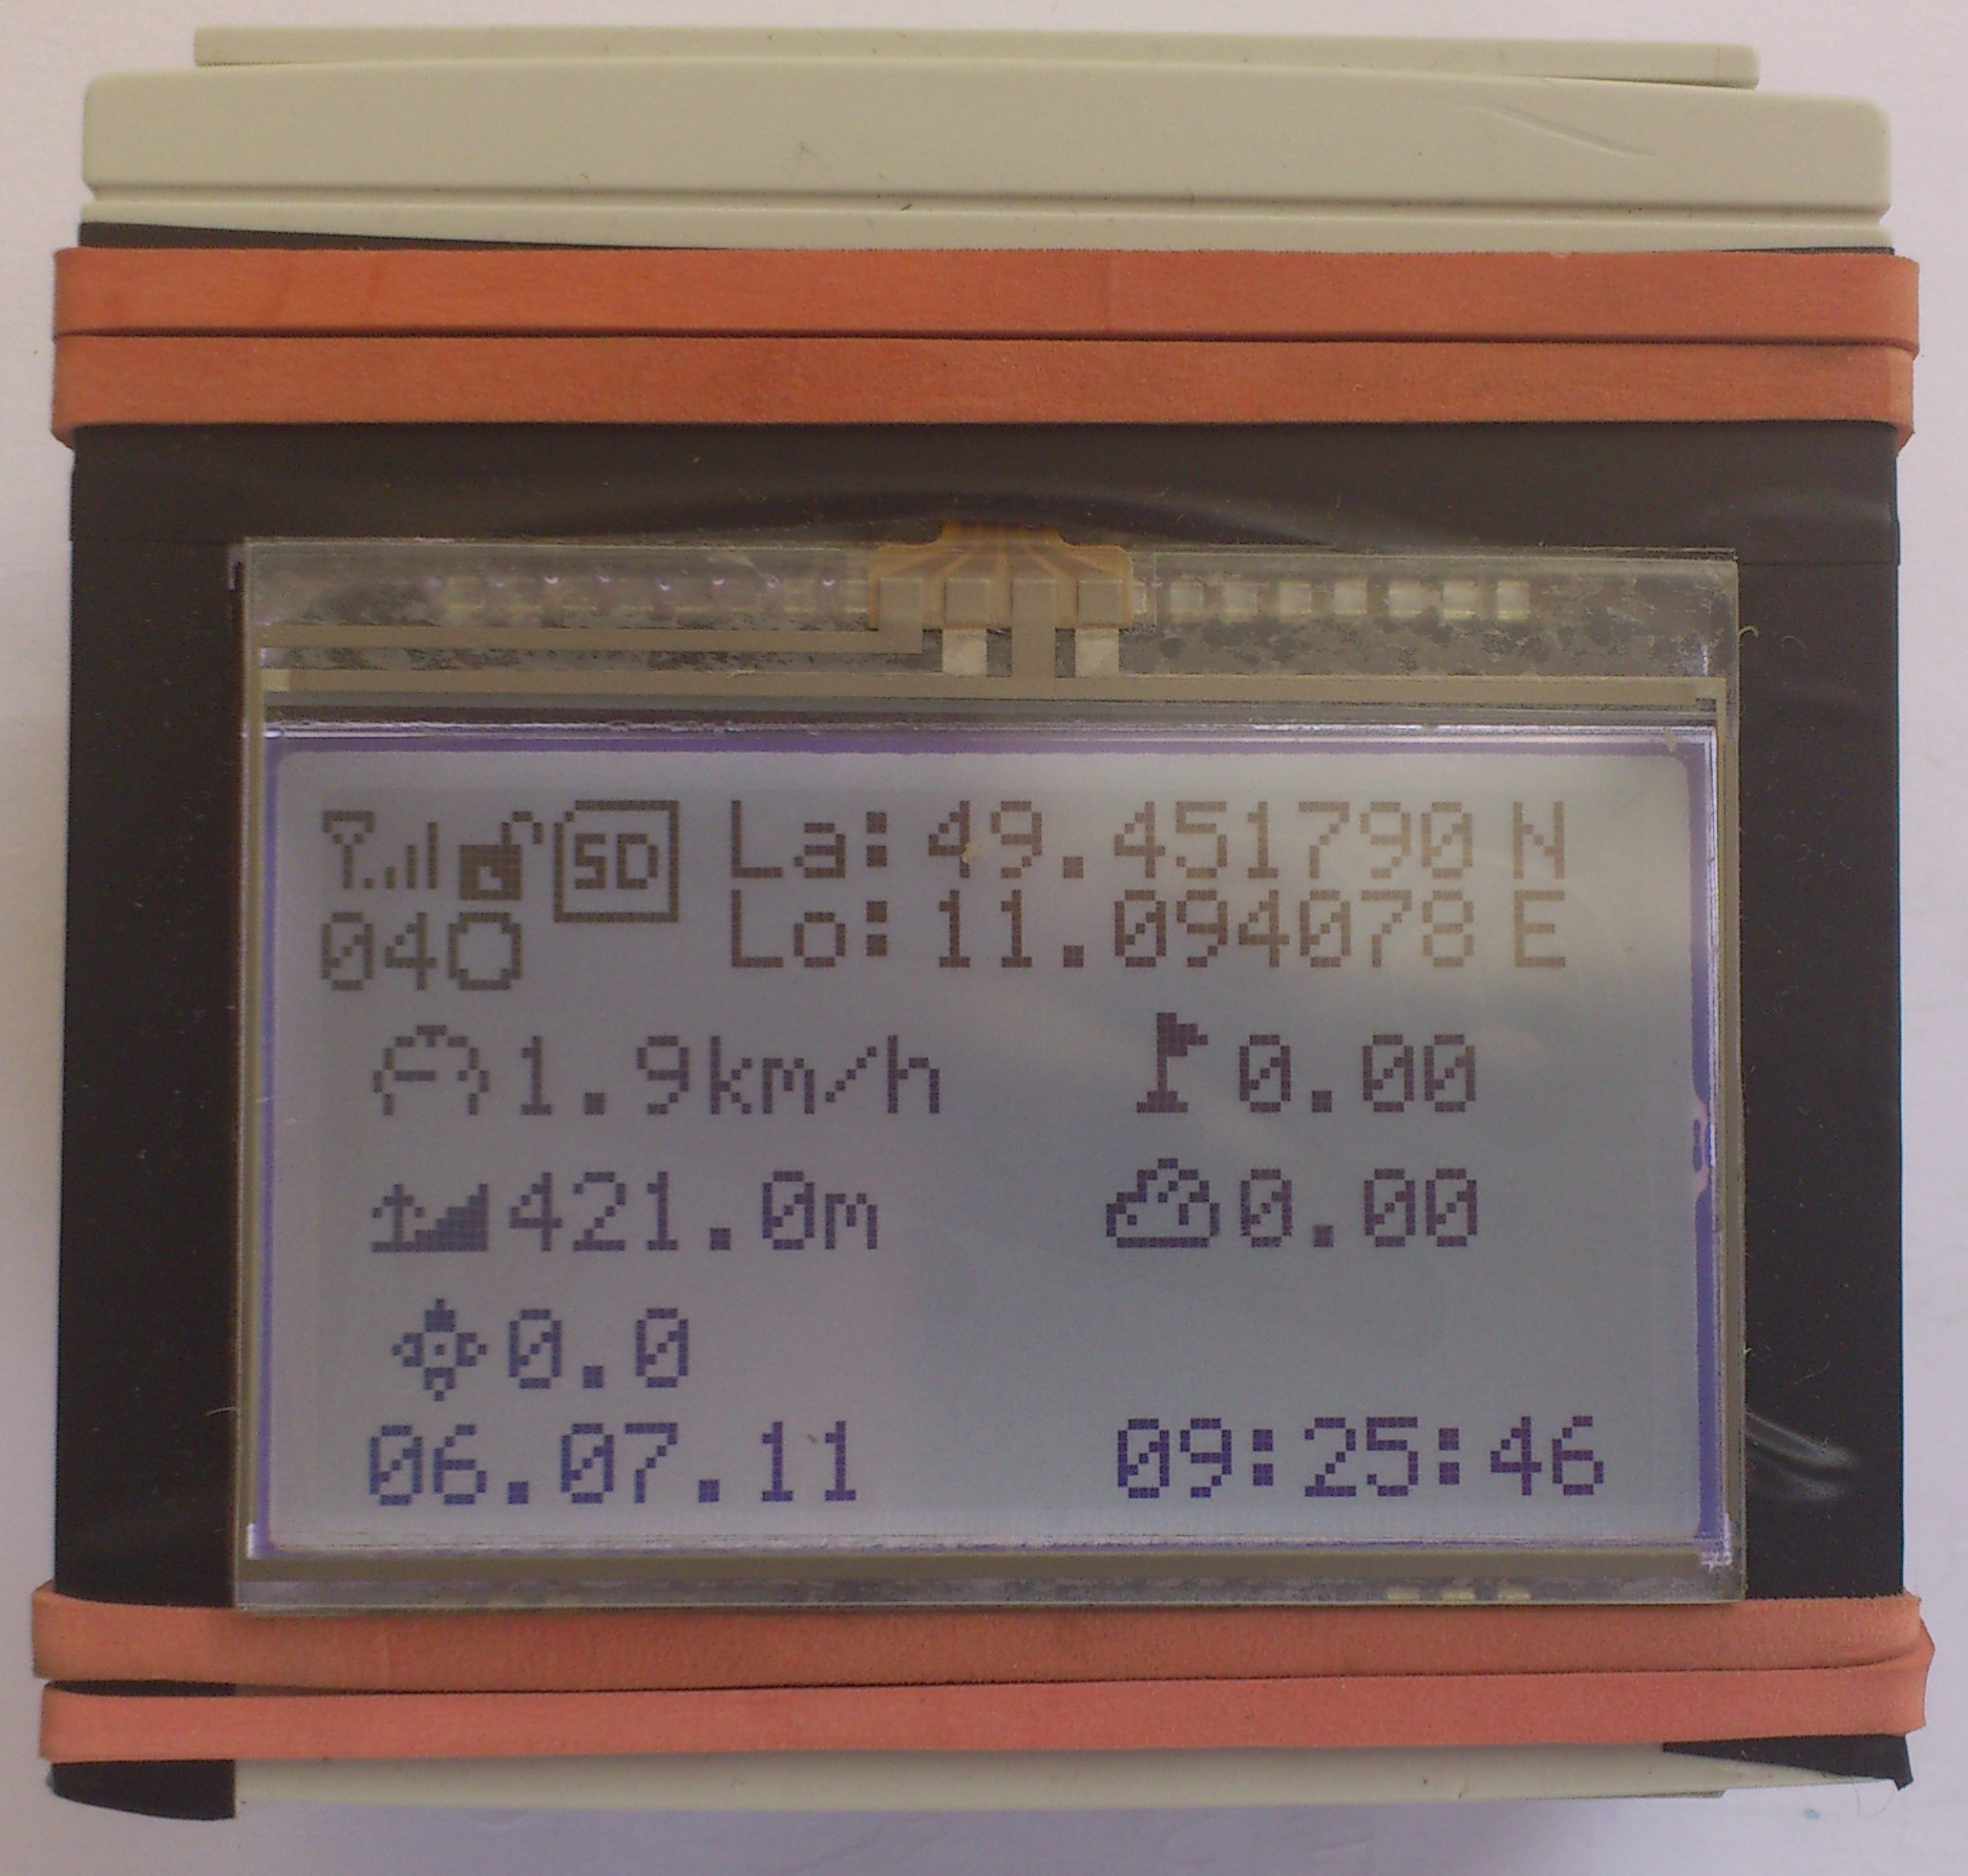
\includegraphics[width=\textwidth]{PIC_recording.pdf}
\captionof{figure}[Recording GPS data]{Recording GPS data}
\label{PIC_record}
\end{minipage}\\

\subsection{Visualization with \texttt{Google Earth}}
The recorded NMEA data sets can be used for a 3D-Visualization by using Google Earth. First of all the NMEA data has to be converted to the
``Keyhole Markup Language" (KML). This is the supported format for Google Earth geographic data. For this you can use ``Wugsis's GPS2KML Converter"
that can be found within the \texttt{tools} directory of the project. After you have copied the recorded data sets from the SD card to your PC,
start \texttt{Wugsi} and push on \texttt{Choose files} within the \texttt{GPS2KML Konverter} tab. Note that the recorded files have a file suffix
\texttt{.NMA}, so you have to adapt the file filter within the \texttt{Open} dialog to \texttt{All files (*.*)}. After loading your file in
\texttt{Wugsi} you can choose some features for the converted \texttt{KML} file, like hight, speed, etc. To actually convert the data simply press
the \texttt{Start} button. Within the logging console on the bottom of the application the file name is printed in which the converted data is
stored (\texttt{Output}) as shown in figure \ref{Wugsi}.\\

Google Earth itself can be downloaded at ``http://www.google.de/intl/de/earth/". After an successful installation simply start the application and
choose \textbf{File}$\rightarrow$\textbf{Open...} and select the converted \texttt{KML} file. For further detailed information about the features
and the services of Google Earth please refer to the official manual. An example of a 3D visualization is shown in figure \ref{google_earth}.\\

\begin{minipage}[t]{\textwidth}
\centering
\includegraphics[width=\textwidth]{Wugsi.pdf}
\captionof{figure}[Wugsi's GPS2KML Converter]{Wugsi's GPS2KML Converter}
\label{Wugsi}
\end{minipage}\\

\begin{minipage}[t]{\textwidth}
\centering
\includegraphics[width=\textwidth]{google_earth.pdf}
\captionof{figure}[3D Visualization within Google Earth]{3D Visualization within Google Earth}
\label{google_earth}
\end{minipage}\\

\newpage 

\section{Developers Guide}
\subsection{Setting up the Hardware}

\begin{enumerate}
\item Remove rubber bands\\
\begin{minipage}[t]{0.5\textwidth}
\centering
\includegraphics[width=\textwidth]{PIC_remove_rubber_bands.pdf}
\label{PIC_remove_rubber_bands}
\end{minipage}\\

\item Open the device
\item Remove clips and connector\\
\begin{minipage}[t]{0.5\textwidth}
\centering
\includegraphics[width=\textwidth]{PIC_remove_connector.pdf}
\label{PIC_remove_connector}
\end{minipage}
\begin{minipage}[t]{0.5\textwidth}
\centering
\includegraphics[width=\textwidth]{PIC_remove_clips.pdf}
\label{PIC_remove_clips}
\end{minipage}\\
\item plug in external supply voltage and programming device. Be absolutely sure that the black cable is \texttt{�} and the yellow one is 
\texttt{+}! Supply voltages 5.5 V � 9 V. Next to the SD Slot is the ISP connector. Next to the voltage jack is the JTAG connector. For JTAG a 
JTAG controller is needed who is compliant with the ATMega644.\\
\begin{minipage}[t]{0.5\textwidth}
\centering
\includegraphics[width=\textwidth]{PIC_plugin_external_voltage.pdf}
\label{PIC_plugin_external_voltage}
\end{minipage}\\
\end{enumerate}

\subsection{Software Setup}
\begin{itemize}
\item Extract the Linux Image debian.rar provided on the DVD
\item Download VirtualBox: http://www.virutalbox.org/wiki/Downloads, and set up Virtualbox with the provided Linux Image. Also set up a filter for the ISP or JTAG Programmer.\\
\begin{minipage}[t]{\textwidth}
\centering
\includegraphics[width=\textwidth]{VirtualBox.pdf}
\label{VirtualBox}
\end{minipage}\\
\begin{minipage}[t]{\textwidth}
\centering
\includegraphics[width=\textwidth]{virtualbox_filter.pdf}
\label{virtualbox_filter}
\end{minipage}\\
\item Boot the Linux Image and login with user dev:
\begin{itemize}
\item \textbf{user:} dev
\item \textbf{password:} dev
\item \textbf{root:} linux
\end{itemize}
\item The directory structure of the home directory of user \texttt{dev}:
\begin{itemize}
\item \texttt{src} contains the source code
\item \texttt{hw} contains hardware circuit and layout files
\item \texttt{doc} contains the documentation of the project
\item \texttt{doxygen} contains the API documentation
\item \texttt{tools} contains some tools used
\item \texttt{stubs} contains some code stubs
\item \texttt{mfile} is a program that creates initial Makefiles
\end{itemize}
\item Plug-in the ISP Programmer; VirtualBox should connect it automatically due to the filter. With the Strange Distribution Diamex ISP Programmer the device is \texttt{/dev/ttyACM0}\\
\begin{minipage}[t]{\textwidth}
\centering
\includegraphics[width=0.8\textwidth]{ISP_programmer.pdf}
\label{ISP_programmer}
\end{minipage}\\
\item If you are not using the Diamex DX-10 ISP Programmer you need to make changes in \texttt{src/Makefile} with the AVRDUDE\_PORT and the AVRDUDE\_PROGRAMMER.\\\textbf{Note:} See avrdude man-pages which protocol you need for your programmer.
\item type \texttt{cd ~/src} and \texttt{make}: The whole source tree is built and if successfully compiled the binary the device will be programmed.
\item After make has sucessfully built the source and programmed the device it gives the following messages:\\
\begin{minipage}[t]{\textwidth}
\centering
\includegraphics[width=0.8\textwidth]{positive_message.pdf}
\label{positive_message}
\end{minipage}\\
\item If you get an error like this check the permissions of the programmer for your user\\
\begin{minipage}[t]{\textwidth}
\centering
\includegraphics[width=0.8\textwidth]{permission_denied.pdf}
\label{permission_denied}
\end{minipage}\\
\item If you get an error like this, be sure if the target does not have any short circuits\\
\begin{minipage}[t]{\textwidth}
\centering
\includegraphics[width=0.8\textwidth]{invalid_signature.pdf}
\label{invalid_signature}
\end{minipage}\\
\item If you get errors like this be sure if the target is connected to the supply voltage\\
\begin{minipage}[t]{\textwidth}
\centering
\includegraphics[width=0.8\textwidth]{lfuse_changed.pdf}
\label{lfuse_changed}
\end{minipage}\\
\item If you get errors like this, the ISP Programmer needs to be reseted. In order to do that, simply unplug and reconnect it to the PC.\\
\begin{minipage}[t]{\textwidth}
\centering
\includegraphics[width=0.8\textwidth]{timeout.pdf}
\label{timeout}
\end{minipage}\\
\item If you get errors like this make sure the programmer is connected to the computer and the AVRDUDE\_PORT is correct in Makefile\\
\begin{minipage}[t]{\textwidth}
\centering
\includegraphics[width=0.8\textwidth]{open_device.pdf}
\label{open_device}
\end{minipage}\\
\item If you get errors like this, make sure the AVRDUDE\_PROGRAMMER is correct in the Makefile\\
\begin{minipage}[t]{\textwidth}
\centering
\includegraphics[width=0.8\textwidth]{claim_device.pdf}
\label{claim_device}
\end{minipage}\\
\item Without errors the device is now successfully programmed.\\\textbf{Note:} We only support the Diamex DX-10 ISP Programmer. Other ISP or JTAG programmers are untested but should work just fine.
\end{itemize}

\appendix
\section{Optional features for future development}
There are a lot of possibilities to improve/extend this project. First of all the implementation of an OS would be a major improvement. Using this feature complex user interaction via touchscreen would be possible.

\section{Known Bugs}
\begin{itemize}
\item The graphical notification that indicates whether a SD card is inserted and writable or not, does not work properly.
\item In every SD card data record a \texttt{$\$ G\backslash n\backslash r$} is received. But this has no effect on the actual functionality of \texttt{Wugsi}
\item The distance calculation does not work properly.
\end{itemize}

\newpage 
\begin{thebibliography}{100}
\bibitem[EADOGL08]{EADOGL} Electronic Assembly, ``DOGL GRAFIK SERIE", 2008, http://www.lcd-module.de/pdf/grafik/dogl128-6.pdf
\bibitem[NAVLOK09]{NAVLOK} u-blox 5, ``NAVILOCK Datenblatt", 2009
\bibitem[NMEA08]{NMEA} u-blox 5, ``NMEA, PUBX Protocol Specification", 2008
\bibitem[AVRTUT09]{AVRGCC} www.Microcontroller.net, ``AVR-GCC-Tutorial", 2009, http://www.mikrocontroller.net/articles/AVR-GCC-Tutorial
\end{thebibliography}
\end{document}